\subsection{Modifica dataset salvati}

\begin{figure}[H]
    \centering
    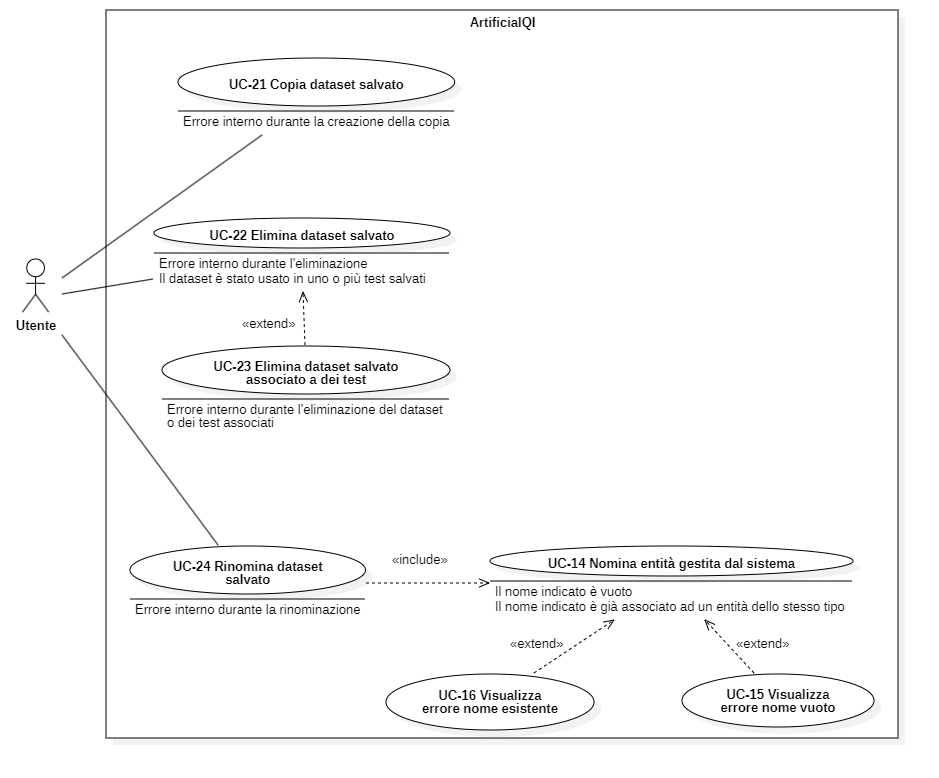
\includegraphics[scale=0.2]{Sezioni/UseCase/Immagini/ModificaDatasetSalvato.png}
    \caption{Diagramma modifica dataset salvati.}
\end{figure}

\begin{usecase}{UC-24}{Copia dataset salvato}
    \label{uc:UC-24}
    
    \req{\hyperref[ru:RUO-3]{RUO-3}} 

    \pre{
        \item L'utente sta visualizzando i dataset salvati \hyperref[uc:UC-22]{UC-22}
    }

    \post{
        \item Il sistema crea una copia del dataset salvato
    }
    
    \actor{Utente}

    \subactors{}

    \trigger{L'utente vuole creare una copia di un dataset salvato}

    \inc{}

    \base{}

    \scenario{
        \item L'utente richiede di copiare un dataset salvato
        \item Il sistema crea una copia del dataset salvato avente nome predefinito
        \item Il sistema notifica l'utente che la copia è andata a buon fine
    }

    \subscenario{
        \item[2.1] Avviene un errore interno al sistema durante la creazione della copia:
        \begin{itemize}
            \item \hyperref[uc:UC-16]{UC-16}
        \end{itemize}
    }
\end{usecase}


\begin{usecase}{UC-25}{Elimina dataset salvato}
    \label{uc:UC-25}
    
    \req{\hyperref[ru:RUO-3]{RUO-3}} 

    \pre{
        \item L'utente sta visualizzando i dataset salvati
    }

    \post{
        \item Il sistema elimina il dataset salvato che è quindi irrecuperabile
    }
    
    \actor{Utente}

    \subactors{}

    \trigger{L'utente richiede l'eliminazione di un dataset salvato}

    \inc{}

    \base{}

    \scenario{
        \item L'utente specifica il dataset salvato da eliminare
        \item Il sistema verifica che non esistano test che hanno utilizzato una qualsiasi versione del dataset
        \item Il sistema richiede la conferma dell'eliminazione
        \item L'utente conferma l'eliminazione
        \item Il sistema elimina il dataset salvato
        \item Il sistema avvisa l'utente della corretta eliminazione
    }
    \subscenario{
        \item[2.1] Il dataset da eliminare è stato usato nella sua versione attuale o nelle precedenti in uno o più test salvati:
        \begin{itemize}
            \item \hyperref[uc:UC-26]{UC-26}
        \end{itemize}
        \item[4.1] L'utente annulla l'operazione di eliminazione:
        \begin{itemize}
            \item Il sistema annulla l'operazione
            \item Lo stato del sistema resta invariato
            \item L'utente viene notificato del corretto annullamento
        \end{itemize} 
        \item[5.1] Avviene un errore interno al sistema durante l'eliminazione:
        \begin{itemize}
            \item \hyperref[uc:UC-16]{UC-16}
        \end{itemize}
    }
\end{usecase}

\begin{usecase}{UC-26}{Elimina dataset salvato associato a dei test}
    \label{uc:UC-26}
    
    \req{} 

    \pre{
        \item Il dataset da eliminare è associato a uno o più test
    }

    \post{
        \item Il dataset e i test a esso associati vengono eliminati e sono quindi irrecuperabili
    }
    
    \actor{}

    \subactors{}

    \trigger{Il sistema deve eliminare un dataset associato a uno o più test}

    \inc{}

    \base{}

    \scenario{
        \item Il sistema visualizza la lista di test associati al dataset e avvisa l'utente che verranno eliminati
        \item L'utente conferma l'eliminazione
        \item Il sistema elimina il dataset 
        \item Il sistema elimina i test associati
        \item Il sistema avvisa l'utente della corretta eliminazione
    }
    \subscenario{
        \item[2.1] L'utente annulla l'operazione di eliminazione:
        \begin{itemize}
            \item Il sistema annulla l'operazione
            \item Lo stato del sistema resta invariato
            \item L'utente viene notificato del corretto annullamento
        \end{itemize} 
        \item[3.1] Avviene un errore interno al sistema durante l'eliminazione del dataset:
        \begin{itemize}
            \item \hyperref[uc:UC-16]{UC-16}
        \end{itemize}
        \item[4.1] Avviene un errore interno al sistema durante l'eliminazione dei test associati:
        \begin{itemize}
            \item \hyperref[uc:UC-16]{UC-16}
        \end{itemize}
    }
\end{usecase}

\begin{usecase}{UC-27}{Rinomina dataset salvato}
    \label{uc:UC-27}
    
    \req{\hyperref[ru:RUO-3]{RUO-3}} 

    \pre{
        \item L'utente sta visualizzando i dataset salvati \hyperref[uc:UC-22]{UC-22}
    }

    \post{
        \item Il sistema rinomina il dataset salvato indicato
    }
    
    \actor{Utente}

    \subactors{}

    \trigger{L'utente vuole rinominare un dataset salvato}

    \inc{\hyperref[uc:UC-17]{UC-17}}

    \base{}

    \scenario{
        \item L'utente richiede di rinominare un dataset salvato
        \item Il sistema ottiene il nuovo nome seguendo \hyperref[uc:UC-17]{UC-17}
        \item L'utente conferma la rinominazione
        \item Il sistema rinomina il dataset salvato
    }

    \subscenario{
        \item[3.1] L'utente annulla la rinominazione:
        \begin{itemize}
            \item Il sistema interrompe l'operazione
        \end{itemize}
        
        \item[4.1] Avviene un errore interno al sistema durante la rinominazione:
        \begin{itemize}
            \item \hyperref[uc:UC-16]{UC-16}
        \end{itemize}
        
    }
\end{usecase}

